\documentclass[letterpaper,10pt]{article}
\usepackage[pdftex]{graphicx}
\usepackage{listings}
\usepackage{alltt}
\usepackage{color}
\usepackage[colorlinks,linkcolor=blue]{hyperref}

\definecolor{dkgreen}{rgb}{0,0.6,0}
\definecolor{gray}{rgb}{0.5,0.5,0.5}
\definecolor{mauve}{rgb}{0.58,0,0.82}

\lstset{
	basicstyle=\footnotesize,
	breaklines=true,
}


\begin{document} 

\begin{titlepage}

\begin{center}

\Huge{Assignment 2}

\Large{CS532-s16:  Web Sciences}

\Large{Spring 2016}

\Large{John Berlin}

\Large Generated on \today

\end{center}

\end{titlepage}
\paragraph{1}
\newpage

\section*{Question 1}
\begin{verbatim}
 Write a Python program that extracts 1000 unique links from Twitter.
 http://thomassileo.com/blog/2013/01/25/using-twitter-rest-api-v1-dot-1-with-python/

 But there are many other similar resources available on the web.  Note
 that only Twitter API 1.1 is currently available; version 1 code will
 no longer work.

 Also note that you need to verify that the final target URI (i.e., the
 one that responds with a 200) is unique.  You could have many different
 shortened URIs for www.cnn.com (t.co, bit.ly, goo.gl, etc.).

 You might want to use the search feature to find URIs, or you can
 pull them from the feed of someone famous (e.g., Tim O'Reilly).

 Hold on to this collection -- we'll use it later throughout the semester. 
\end{verbatim}
\subsection*{Answer}

Extracting a 1000 unique links from Twitter at first seemed like a daunting task. The first steps I took to solving this problem was to look at the libraries twitter themselves suggested for use \href{https://dev.twitter.com/overview/api/twitter-libraries}{Twitter Libraries}. I also did search for blog posts on twitter mining and a tutorial that was most helpful.


The \href{http://marcobonzanini.com/2015/03/02/mining-twitter-data-with-python-part-1/}{tutorial} Mining Twitter Data with Python used the library \verb+Tweepy+ which I was quick to modify for use in this assignment.

To get the uri's use the file \verb+twitter_stream.py+
\begin{enumerate}
\item \verb+twitter_stream.py+ \textless -q\textgreater \textless the query\textgreater 
	\begin{itemize}
	\item Takes a query to look for in the twitter stream
	\item Connect to the twitter stream and listen
	\item On Tweet that matches query get the json data
	\item Extract the uri using the expanded url field
	\item Append the uri to the file
	\item Code in listing \ref{lst:q1TwitterStreaming} starting on page \pageref{lst:q1TwitterStreaming}:
	\end{itemize}
\end{enumerate}
\newpage 
\lstinputlisting[language=Python,
frame=single,
caption={Python program to mine urls for a twitter query},label=lst:q1TwitterStreaming,captionpos=b,numbers=left,
numberstyle=\tiny\color{gray},keywordstyle=\color{blue},
  commentstyle=\color{dkgreen}, stringstyle=\color{mauve},showspaces=false,showstringspaces=false,basicstyle=\footnotesize]{twitter_stream.py}
 \newpage  
\section*{Question 2}
\begin{verbatim}
 Download the TimeMaps for each of the target URIs.  We'll use the ODU 
Memento Aggregator, so for example:

URI-R = http://www.cs.odu.edu/

URI-T = http://mementoproxy.cs.odu.edu/aggr/timemap/link/1/http://www.cs.odu.edu/

Create a histogram* of URIs vs. number of Mementos (as computed from
the TimeMaps).  For example, 100 URIs with 0 Mementos, 300 URIs
with 1 Memento, 400 URIs with 2 Mementos, etc.

* = https://en.wikipedia.org/wiki/Histogram 
\end{verbatim}
\subsection*{Answer}
To answer this question and the last one I combined the steps to generate the required data into as few files as possible. The following steps give a break down to use the files with detail into what is going on is provided as comments in the code 
\begin{enumerate}
\item run \verb+local.py+ from the carbon date library 
	\begin{itemize}
	\item use method \verb+uniques+ and \verb+zeroNoneZero+ from \verb+util.py+ to ensure the selected uris are unique, also to generate the nonzero uri file
	\item copy the file nonzero.txt to the directory containing the Carbon Dating library with modified local.py
	\item The file used to provide the timemap support was originally written by Scott Ainsworth which I modified to be compatible with python3. It is found in listing  \ref{lst:tmaps} starting on page \pageref{lst:tmaps}. The number of mementos is the length of the keys to memento map in TimeMap class contained in this file
	\item run and copy dumped json file called dated.json back to location where \verb+carbonDating.py+ is
	\item Code in listing \ref{lst:local} starting on page \pageref{lst:local}
	\end{itemize}
\item \verb+carbonDating.py+
	\begin{itemize}
	\item Count the number of Mementos per uri if there is an exception there are no mementos for the uri so associate a count of 0 with that uri
	\item Parse the json file dated.json with the uri's in contained in the nonezero file produced by running the \verb+zeroNoneZero+ from \verb+util.py+
	\item the age of the memento is the python Date delta from today to age gotten from running the modified \verb+local.py+ in listing \ref{lst:local} starting on page \pageref{lst:local} from the CarbonDating library 
	\item Code in listing \ref{lst:cDate} starting on page \pageref{lst:cDate}
	\end{itemize}
\end{enumerate}
The R script to generate the figure \ref{fig:bt1} shows the histogram of the mementos counts
is found is shown below.

\lstinputlisting[language=R,
frame=single,
caption={Memento Count HistoGram R script},label=lst:mHisto,captionpos=b,numbers=left,
numberstyle=\tiny\color{gray},keywordstyle=\color{blue},
  commentstyle=\color{dkgreen}, stringstyle=\color{mauve},showspaces=false,showstringspaces=false,basicstyle=\footnotesize]{mementoCountHistogram.R}
    
\begin{figure}[!ht]
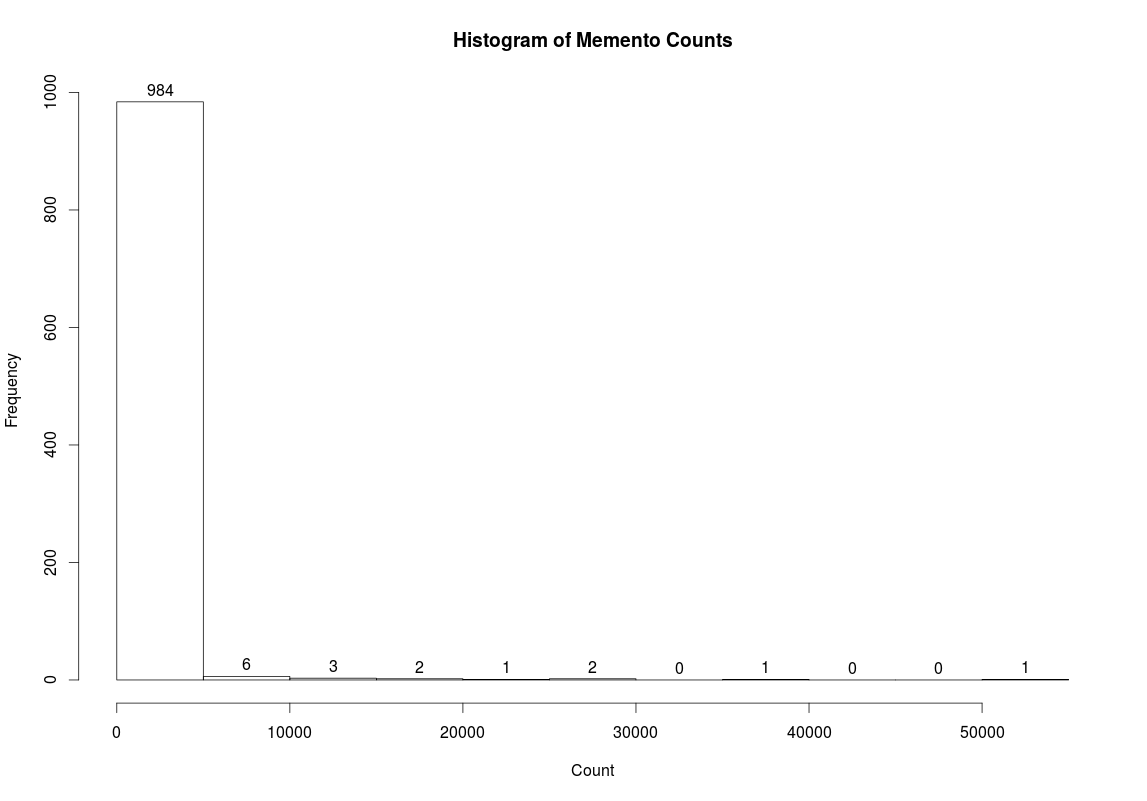
\includegraphics[scale=0.3]{images/CountHist.png}
\caption{histogramCounts}
\label{fig:bt1}
\end{figure}

As seen in the Histogram there were more uris with less than 1000 mementos

 \newpage  
\lstinputlisting[language=Python,
frame=single,
caption={TimeMaps},label=lst:tmaps,captionpos=b,numbers=left,
numberstyle=\tiny\color{gray},keywordstyle=\color{blue},
  commentstyle=\color{dkgreen}, stringstyle=\color{mauve},showspaces=false,showstringspaces=false,basicstyle=\footnotesize]{timemaps.py} 
\newpage    
\lstinputlisting[language=Python,
frame=single,
caption={util},label=lst:utils,captionpos=b,numbers=left,
numberstyle=\tiny\color{gray},keywordstyle=\color{blue},
  commentstyle=\color{dkgreen}, stringstyle=\color{mauve},showspaces=false,showstringspaces=false,basicstyle=\footnotesize]{util.py}  
 \newpage  
\lstinputlisting[language=Python,
frame=single,
caption={Modified local.py},label=lst:local,captionpos=b,numbers=left,
numberstyle=\tiny\color{gray},keywordstyle=\color{blue},
  commentstyle=\color{dkgreen}, stringstyle=\color{mauve},showspaces=false,showstringspaces=false,basicstyle=\footnotesize]{local.py}

\newpage  
\lstinputlisting[language=Python,
frame=single,
caption={Python program to mine urls for a twitter query},label=lst:cDate,captionpos=b,numbers=left,
numberstyle=\tiny\color{gray},keywordstyle=\color{blue},
  commentstyle=\color{dkgreen}, stringstyle=\color{mauve},showspaces=false,showstringspaces=false,basicstyle=\footnotesize]{carbonDating.py}
\section*{Question 3}
\begin{verbatim}
Estimate the age of each of the 1000 URIs using the "Carbon Date" tool:

http://ws-dl.blogspot.com/2014/11/2014-11-14-carbon-dating-web-version-20.html

Note: you'll should download the library and run it locally; don't
try to use the web service.

For URIs that have > 0 Mementos and an estimated creation date,
create a graph with age (in days) on one axis and number of mementos
on the other.  

Not all URIs will have Mementos, and not all URIs will have an estimated
creation date.  State how many fall into either categories. 
\end{verbatim}
\subsection*{Answer}

Out of the 1000 uri mementos 28 of them were found to have an age of 0 but none of the uri were found to have a memento count of 0.   

Using the generated files from the python files I used R code found in listing \ref{lst:mAgeCount} starting on page \pageref{lst:mAgeCount} to generate figure \ref{fig:bt2}.

In the r script I found the median memento count and partitioned the data frame into two halves those that fell below the median and those the fall about it. This was to have two graphs that clearly show the entire graph.

The number of mementos that were above the median are fare more dispersed than those below it. As seen in the all age count graph it is difficult to see the distribution due to outliers. 

\begin{figure}[!ht]
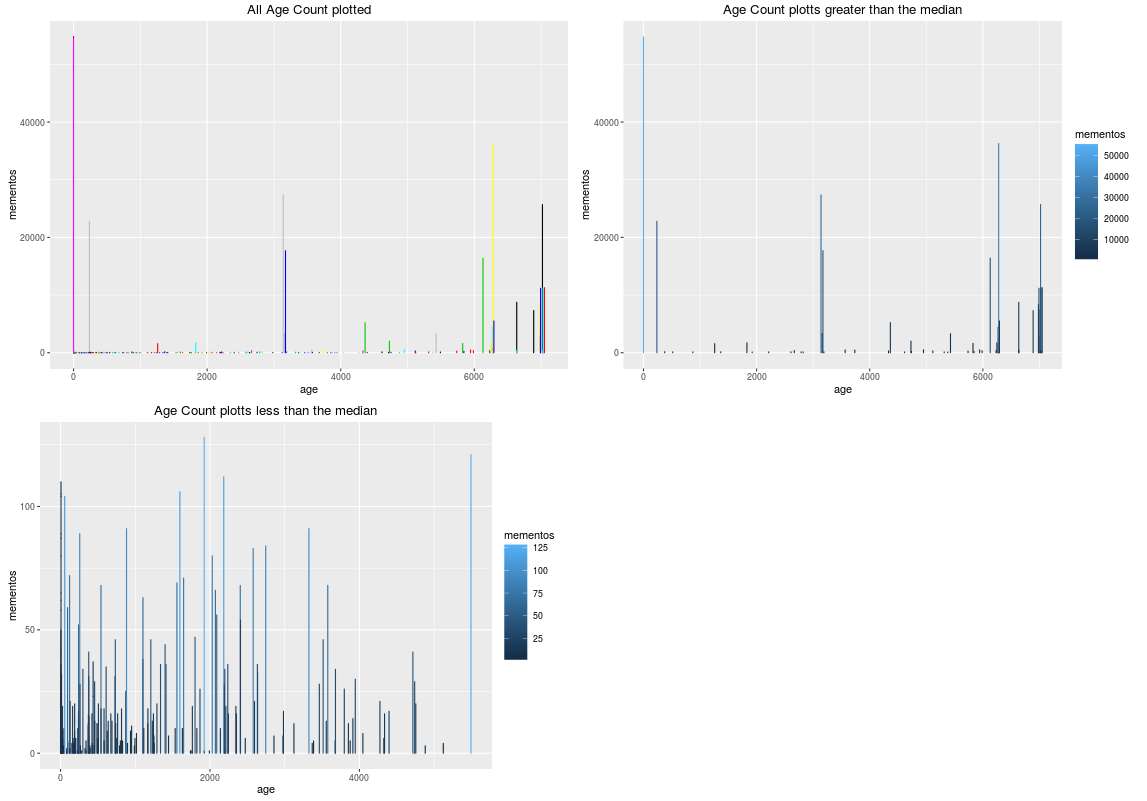
\includegraphics[scale=0.4]{images/ageCount.png}
\caption{histogramCounts}
\label{fig:bt2}
\end{figure}
  
\lstinputlisting[language=R,
frame=single,
caption={Memento Count Age R script},label=lst:mAgeCount,captionpos=b,numbers=left,
numberstyle=\tiny\color{gray},keywordstyle=\color{blue},
  commentstyle=\color{dkgreen}, stringstyle=\color{mauve},showspaces=false,showstringspaces=false,basicstyle=\footnotesize]{mementoCountAge.R}

        
\end{document}